\section{Алгоритм Чена—Хана}

\begin{frame}{Постановка задачи}
	Дана поверхность многогранника; все грани~— треугольники.\\
	Выбрана вершина \(S\). Найти длины кратчайших \\
	путей {\it (по поверхности многогранника)} от \(S\) \\
	до каждой из остальных его вершин.
\end{frame}


\begin{frame}{Устройство кратчайших путей}
   \begin{itemize}
	\item Кратчайший путь переходит с грани на грань\\
		не более \(n-1\) раза,\medskip
	\item Кратчайшие пути не пересекаются, кроме как\\
		в \(S\) или в вершине назначения,\medskip
	\item При разгибании рёбер кратчайший путь превращается\\
		в отрезок прямой линии.
   \end{itemize}
\end{frame}


\begin{frame}{Дерево кратчайших путей}
	Грани многогранника хранятся в DCEL; путь определяется\\
	последовательностью пройденных граней.

	Покажем, как пересчитываются пути при переходе\\
	на следующую грань и как формируется двоичное дерево.
\end{frame}


\begin{frame}{One angle — one split}
   \begin{lm}
	Из двух узлов дерева, расположенных на одном полуребре,\\
	только у одного может быть два потомка,\\
	определяющих кратчайшие пути.
   \end{lm}
\end{frame}


\begin{frame}{Эффективный алгоритм}
	Считаем двух детей листа и проверяем, кто теперь\\
	{\it оккупирует} вершину многогранника под ним. У того,\\
	кто {\it (теперь)} не оккупирует, удаляем одного ребёнка.

	На каждой итерации у дерева линейное количество листьев:\\
	по одному на каждое полуребро, плюс по одному \\
	разделяющемуся на каждое полуребро.

	Глубина дерева \alert{не более \(n\).}
\end{frame}


\section{Теорема Александрова}

\begin{frame}{Отношение эквивалентности}
	Дан набор многоугольников. Разобьём \(\bigcup \partial P_i\) на отрезки,\\
	пары отрезков одинаковой длины можно\\
	склеивать между собой.

	Будем рассматривать \alert{фактор-пространство,} получающееся\\
	при таком склеивании.
\end{frame}


\begin{frame}{Теорема Александрова: склейки}
	Нас интересуют склейки, которые гомеоморфны сфере и\\
	угол в каждой точке которых не превосходит \(360^\circ\).
\begin{figure}
	\centering
	\begin{subfigure}[m]{0.41\textwidth}
		\centering
		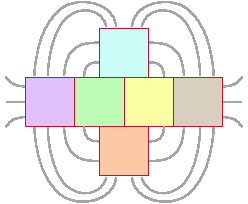
\includegraphics[scale=1.12]{figs_pres/alex_example_1}
	\end{subfigure}
~
	\centering
	\begin{subfigure}[m]{0.48\textwidth}
		\centering
		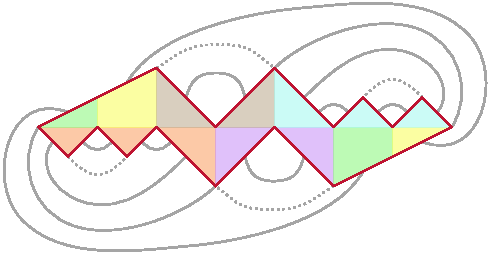
\includegraphics[scale=0.81]{figs_pres/alex_example_stefan_1}
	\end{subfigure}
\end{figure}
\end{frame}


\begin{frame}{Теорема Александрова: многогранники} \ \\
\begin{thm}
	Склейке, удовлетворяющей этим условиям, соответствует\\
	(изометричен) единственный выпуклый многогранник.
\end{thm} \medskip
\begin{figure}
	\centering
	\begin{subfigure}[m]{0.38\textwidth}
		\centering
		\tikz{\begin{scope}[scale=0.86] % [scale=0.62]
% \filldraw[draw=white,fill=white] (0, 1.25 + 0.45 - 2.4) rectangle (3.6 ,1.25 + 0.45 + 2.4);

\draw[color=thr] (0,0) -- (1.1,0.9) -- ++(0,2.5);
\draw[color=thr] (1.1,0.9) -- ++(2.5,0);

\draw [thick,color=edThr, dashed] (0.55,0.45) -- ++(0,2.5);
\draw [thick,color=edThr, dashed] (1.1 cm + 1.25 cm, 0.9) -- ++(0,2.5);
\draw [thick,color=edThr, dashed] (0,0) -- (1.1,0.9) -- ++(2.5,0);

\zal 4 (2.5,2.5) -- ++(1.1,0.9) -- ++(-2.5,0) -- ++(-1.1,-0.9) -- cycle;
\zal 6 (2.5 cm + 0.55 cm,0.45) -- ++(0.55,0.45) -- ++(0,2.5) -- ++(-0.55,-0.45) -- cycle;
\zal 3 (0,0) -- ++(1.25,0) -- ++(0,2.5) -- ++(-1.25,0) -- cycle;
\zal 2 (1.25,0) -- ++(1.25,0) -- ++(0.55,0.45) -- ++(0,2.5) -- ++(-0.55,-0.45) -- ++(-1.25,0) -- cycle;

\draw[dgray] (0,0) -- (0,2.5) -- (2.5,2.5) -- (2.5,0) -- cycle;
\draw[dgray] (2.5,0) -- ++(1.1,0.9) -- ++(0,2.5) -- ++(-1.1,-0.9) -- cycle;
\draw[dgray] (2.5,2.5) -- ++(1.1,0.9) -- ++(-2.5,0) -- ++(-1.1,-0.9) -- cycle;

\draw [thick,color=edHr] (1.25,0) -- ++(0,2.5);
\draw [thick,color=edHr] (2.5 cm + 0.55 cm, 0.45) -- ++(0,2.5);
\draw [thick,color=edHr] (2.5,2.5) -- ++(1.1,0.9) -- ++(-2.5,0) -- ++(-1.1,-0.9) -- cycle;
\draw [thick,color=edHr] (0,0) -- (2.5,0) -- ++(1.1,0.9);
\end{scope}}
	\end{subfigure}
~
	\centering
	\begin{subfigure}[m]{0.38\textwidth}
		\centering
		\tikz{
\begin{scope}[scale=0.86] % [scale=0.62]
% \filldraw[draw=white,fill=white] (0, 1.25 + 0.45 - 2.4) rectangle (3.6 ,1.25 + 0.45 + 2.4);

\draw[color=thr] (0,0) -- (1.1,0.9) -- ++(0,2.5);
\draw[color=thr] (1.1,0.9) -- ++(2.5,0);

\draw [thick,color=edThr, dashed] (0,0) -- (1.1, 0.9 + 2.5);
\draw [thick,color=edThr, dashed] (1.1,0.9) -- ++(2.5,2.5);
\draw [thick,color=edThr, dashed] (0,0) -- (1.1+2.5, 0.9);
\draw [thick,color=edThr, dashed] (2.5,0) -- (1.8,0.45);

\zall 4 (0,2.5) -- ++(2.5,0) -- ++(1.1,0.9) -- ++(-2.5,0) -- cycle;
\zall 3 (0,0) -- (0,2.5) -- (2.5,2.5) -- (2.5,0) -- cycle;
\zall 2 (2.5,0) -- ++(1.1,0.9) -- ++(0,2.5) -- ++(-1.1,-0.9) -- cycle;

\draw[dgray] (0,0) -- (0,2.5) -- (2.5,2.5) -- (2.5,0) -- cycle;
\draw[dgray] (2.5,0) -- ++(1.1,0.9) -- ++(0,2.5) -- ++(-1.1,-0.9) -- cycle;
\draw[dgray] (2.5,2.5) -- ++(1.1,0.9) -- ++(-2.5,0) -- ++(-1.1,-0.9) -- cycle;

\draw [thick,color=edHr] (0,0 +2.5) -- (1.1+2.5, 0.9 +2.5);
\draw [thick,color=edHr] (2.5,0 +2.5) -- (1.8,0.45 +2.5);
\draw [thick,color=edHr] (0,0) -- (2.5,1.25) -- (2.5+1.1,0.9+2.5);

%\draw (0,0) node[left]{$E$};
%\draw (0,2.5) node[left]{$A$};
%\draw (1.1,3.4) node[above]{$B$};
%\draw (1.1+2.5,3.4) node[right]{$C$};
%\draw (1.1+2.5,0.9) node[right]{$G$};
%\draw (2.5,0) node[below]{$H$};
\end{scope}
}
	\end{subfigure}
\end{figure}
\end{frame}
